\documentclass[../../main.tex]{subfiles}

\begin{document}

\section{Markov Chains}

A \textbf{Markov Chain} is a stochastic process $\{X_n\}_{n=0}^\infty$ defined on a discrete state space $S$ such that the probability of transitioning to the next state depends only on the present state and not on the sequence of events that preceded it. This property is known as the \emph{Markov property}. For simplicity's sake, we assume $S$ to be finite. Hence, the formal definition:



\begin{definition}[Markov Chain]
A \textbf{Markov Chain} is a stochastic process $\{X_n\}_{n=0}^\infty$ on a discrete finite state space $S = \{1, \dots , N\}$ satisfying the \emph{Markov property}:
\[
    P(X_{n+1} = x_{n+1} \mid X_n = x_n, \dots, X_0 = x_0) = P(X_{n+1} = x_{n+1} \mid X_n = x_n) \quad ,
\]
for all $n \geq 0$ and all $x_0, \dots, x_{n+1} \in S$.

\noindent
The transition probabilities are described by a matrix $\bm{P}$ with entries
\[
    \bm{P}_{ij} = P(X_{n+1} = i \mid X_n = j), \quad \text{where } \sum_{i \in S} \bm{P}_{ij} = 1 \text{ for all } j \in S.
\]
\end{definition}


\begin{example}[Markov Transition Matrix]
\label{ex:markov_chain}
Let the state space be $S = \{1, 2, 3\}$. A possible transition matrix $\bm{P}$ is:
\[
\bm{P} =
\begin{bmatrix}
0 & 0.7 & 0 \\
0.5 & 0.3 & 1 \\
0.5 & 0 & 0 \\
\end{bmatrix}
\]
Note that each column sums to 1.
\end{example}


\begin{remark}
    Some sources define $\bm{P'}$ s.t. $\bm{P'}_{ij} = P(X_{n+1} = j \mid X_n = i)$. The only difference is that $\bm{P'} = \bm{P}^T$.
\end{remark}


Based on these simple definitions, we can deduce very useful properties. For example, we can calculate $P(X_{t+n} = i \mid X_t = j)$ algebraically very simple based on the following result:


\begin{lemma}[n-Step Transition Probabilities]
The probability of transitioning from state $j$ to state $i$ in $n$ steps is given by the $(i,j)$-th entry of the matrix power $\bm{P}^n$:
\[
    P(X_{t+n} = i \mid X_t = j) = (\bm{P}^n)_{ij}.
\]
\end{lemma}

\begin{proof}
We prove this by induction on \( n \).

\textbf{Base case:} When \( n = 1 \), we have
\[
    P(X_{t+1} = i \mid X_t = j) = \bm{P}_{ij} = (\bm{P}^1)_{ij}.
\]

\textbf{Inductive step:} Assume the claim holds for \( n = k \), i.e.,
\[
    P(X_{t+k} = i \mid X_t = j) = (\bm{P}^k)_{ij}.
\]
For \( n = k+1 \), using the law of total probability and the Markov property:
\begin{align*}
    P(X_{t+k+1} = i \mid X_t = j) &= \sum_{m \in S} P(X_{t+k+1} = i \mid X_{t+k} = m) \cdot P(X_{t+k} = m \mid X_t = j) \\
    &= \sum_{m \in S} \bm{P}_{im} \cdot (\bm{P}^k)_{mj} \\
    &= (\bm{P} \cdot \bm{P}^k)_{ij} = (\bm{P}^{k+1})_{ij} \quad .
\end{align*}
Hence, by induction, the result holds for all \( n \geq 1 \).
\end{proof}

\begin{lemma}[n-Step Probability Distribution]
    If we have a probability distribution vector $\bm{p}_t$ at time $t$, meaning $(\bm{p}_t)_i = P(X_t = i)$, we get $\bm{p}_{t+n}$ by $\bm{P}^n \bm{p}_t$.
\end{lemma}
\vspace{-2.5em}
\begin{proof}
    \begin{align*}
        (\bm{p}_{t+n})_i &= P(X_{t+n} = i) \\
        &= \sum_{j \in S} P(X_{t+n} = i \mid X_t = j) P(X_t = j) \\
        &= \sum_{j \in S} (\bm{P}^n)_{ij} P(X_t = j) \\
        &= (\bm{P}^n \bm{p}_t)_i
    \end{align*}
\end{proof}


\subsection{Properties}
Markov chains are a very simple model. Thus, we can analyze them thoroughly and investigate their properties. But what could these properties be? Well, we first might want to visualize Markov chains. To this end, we employ a graph $G = (V, E)$ with $V = S$ and $E = \{(u, v) \mid \bm{P}_{vu} \neq 0\}$.

Hence, the Markov chain from example~\ref{ex:markov_chain} can be visualized as in figure~\ref{fig:markov_chain}.

\begin{figure}[h]
    \center
    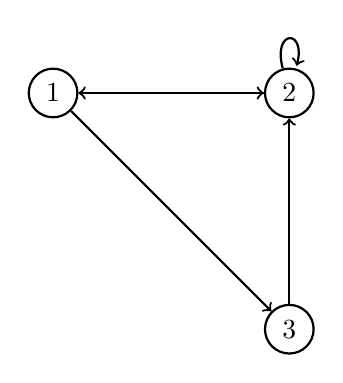
\begin{tikzpicture}[->, auto, node distance=3cm, thick]
    % Define states
    \node[circle, draw] (A) {1};
    \node[circle, draw, right of=A] (B) {2};
    \node[circle, draw, below of=B] (C) {3};

    % Transitions between states
    \draw (A) edge (B);
    \draw (A) edge (C);
    \draw (B) edge (A);
    \draw (C) edge (B);

    % Self-loops
    % \draw (A) edge[loop above] (A);
    \draw (B) edge[loop above] (B);
    % \draw (C) edge[loop below] (C);

    \end{tikzpicture}
    \caption{Graph representation of the Markov chain defined in example~\ref{ex:markov_chain}.}
    \label{fig:markov_chain}
\end{figure}

Note that we do not care about the magnitude of the transition probabilities, it only matters whether it is possible to transition from one state to another.

\subsubsection{Irreducibility}
Already we can see that we can reach every every state $v$ from every other state $u$, i.e. there exists a path of length $n$ starting at $u$ and ending at $v \iff (\bm{P}^n)_{vu} > 0$. Such a Markov chain is called \emph{irreducible}. The importance of this is that the Markov chain cannot trap itself in a subclass of states, like for example in figure~\ref{fig:markov_chain_reducible}.

\begin{figure}[h]
    \center
    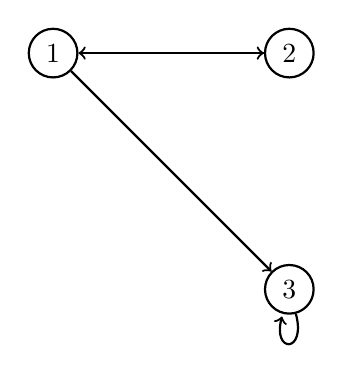
\begin{tikzpicture}[->, auto, node distance=3cm, thick]
    % Define states
    \node[circle, draw] (A) {1};
    \node[circle, draw, right of=A] (B) {2};
    \node[circle, draw, below of=B] (C) {3};

    % Transitions between states
    \draw (A) edge (B);
    \draw (B) edge (A);
    \draw (A) edge (C);

    % Self-loops
    % \draw (A) edge[loop above] (A);
    % \draw (B) edge[loop above] (B);
    \draw (C) edge[loop below] (C);

    \end{tikzpicture}
    \caption{Graph of a reducible Markov chain. Note that once the chain transitions from state $1$ to state $3$, it will stay at state $3$ indefinitely.}
    \label{fig:markov_chain_reducible}
\end{figure}

Before defining this property formally, we may first introduce a very related concept of \emph{communication classes}:

\begin{definition}
    We say that $i \in S$ \emph{leads to} state $j \in S$ iff there exists $n \in \mathbb{N}_{>0}$ s.t. $(\bm{P}^n)_{ji} > 0$. We use the notation $i \leadsto j$. Also, for all $i \in S$: $i \leadsto i$. 
\end{definition}

\begin{definition}[Communication between States]
    States $i,j \in S$ \emph{communicate} iff $i \leadsto j$ and $j \leadsto i$. We use the notation $i \leftrightsquigarrow j$.
\end{definition}

\begin{theorem}
    $i \leftrightsquigarrow j$ is an equivalence relation.
\end{theorem}
\vspace{-2.5em}
\begin{proof}
    Both reflexivity and symmetry follow directly from the definitions. For transitivity we have assuming $i \neq j$ and $j \neq k$ (the other cases are trivial):
    \begin{align*}
        &i \leftrightsquigarrow j \text{ and } j \leftrightsquigarrow k \\
        &\implies i \leadsto j \text{ and } j \leadsto i \\
        &\implies \exists_{m,n \in \mathbb{N}_{>0}} (\bm{P}^m)_{ji} > 0 \text{ and } (\bm{P}^n)_{kj} > 0 \\
        &\implies \exists_{m,n \in \mathbb{N}_{>0}} P(X_m = j \mid X_0 = i) > 0 \text{ and } P(X_{m+n} = k \mid X_m = j) > 0 \\
        &\implies P(X_{m+n} = k \mid X_0 = i) > 0 \\
        &\implies (\bm{P}^{m+n})_{ki} > 0 \\
        &\implies i \leadsto k
    \end{align*}
    $k \leadsto i$ can be show in similar fashion.
\end{proof}

Based on this result, the following definition suggests itself:

\begin{definition}[Communication Class]
    The \emph{communication class} of state $i \in S$ is the set $\{ j \in S : i \leftrightsquigarrow j \}$. This set consists of all states $j$ that communicate with $i$.
\end{definition}

\begin{remark}
    Since communication of states is an equivalence relation, the state space $S$ can be decomposed into a disjoint union of communication classes (also called a \emph{partition}). Any two communication classes either coincide completely or are disjoint sets.
\end{remark}

\begin{example}
    The partition of figure~\ref{fig:markov_chain} is $\{ \{ 1, 2, 3 \} \}$ and of figure~\ref{fig:markov_chain_reducible} we have $\{ \{ 1, 2 \} , \{ 3 \} \}$.
\end{example}

Finally, we can state the concept of \emph{irreducibility} formally:

\begin{definition}[Irreducibility]
    A Markov chain is \emph{irreducible} iff every two states communicate. Hence, an irreducible Markov chain consists of exactly one communication class.
\end{definition}

We will mostly focus on irreducible Markov chains, but for the completeness' sake we also define the following concepts:

\begin{definition}[Open and Closed Communication Class]
    A communication class $C$ is \emph{open} iff there exists a state $i \in C$ and a state $k \not \in C$ s.t. $i \leadsto k$. Otherwise, $C$ is called \emph{closed}.
\end{definition}

\begin{remark}
    An irreducible Markov chain has exactly one closed communication class.
\end{remark}

If a Markov chain once arrived in a closed communication class, it will stay in this class forever. This is exactly what happens in figure~\ref{fig:markov_chain_reducible}.

\begin{theorem}[Existence of Closed Communication Class]
    There is always at least one closed communication class.
\end{theorem}
\vspace{-2.5em}
\begin{proof}
Assume all communication classes $C_1, \dots, C_k$ are open. Hence, we can traverse these classes. But at some point we must complete a cycle, but that is a contradiction, as this would imply that those communication classes forming the cycle are really just one big communication class, which is not the case.
\end{proof}


\subsubsection{Aperiodicity}
We will now analyze the second important property of Markov chains. The reader might ask, \emph{important for what?} Well, the answer will make more sense in the bigger picture later, but the short answer is that these two properties will guarantee for a convergence to a unique stationary probability distribution.

To motivate the following discussion, say we had the following Markov chain:

\begin{figure}[h]
    \center
    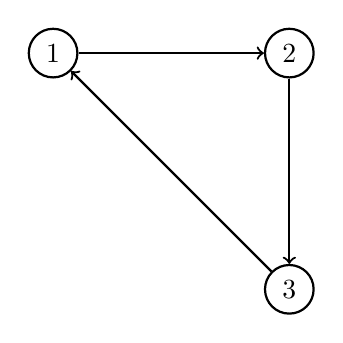
\begin{tikzpicture}[->, auto, node distance=3cm, thick]
    % Define states
    \node[circle, draw] (A) {1};
    \node[circle, draw, right of=A] (B) {2};
    \node[circle, draw, below of=B] (C) {3};

    % Transitions between states
    \draw (A) edge (B);
    \draw (B) edge (C);
    \draw (C) edge (A);

    % Self-loops
    % \draw (A) edge[loop above] (A);
    % \draw (B) edge[loop above] (B);
    % \draw (C) edge[loop below] (C);

    \end{tikzpicture}
    \caption{Graph of a periodic Markov chain. Note that once once the starting position is determined, then we also know the state after $t$ steps.}
    \label{fig:markov_chain_periodic}
\end{figure}

We notice that the behavior of this chain is periodic with a period of length $3$. Of course, this is very informal speaking, but we will now define this idea precisely.

\begin{definition}[Period and Aperiodicity]
    The \emph{period} of state $i \in S$ is defined as
    \[ \gcd \{ n \in \mathbb{N}_{>0} : (\bm{P}^n)_{ii} > 0 \} \quad . \]
    Here, $\gcd$ stands for the greatest common divisor. A state $i \in S$ is called aperiodic iff its period is equal to $1$. Otherwise, the state $i$ is called periodic.
\end{definition}

\begin{remark}
    This definition is not well defined in all cases, as it could happen that $\{ n \in \mathbb{N}_{>0} : (\bm{P}^n)_{ii} > 0 \} = \emptyset$. However, we mostly care about Markov chains being aperiodic in closed communication classes, especially in irreducible Markov chains. And for closed communication classes, this set can never be empty. In fact, for the set to be empty, we must have a communication class consisting of only one state $i \in S$ with $\bm{P}_{ii} = 0$. This communication class is obviously open.
\end{remark}

\begin{lemma}[Periodicity and Aperiodicity are Class Properties]
    If state $i \in S$ is aperiodic and $i \leftrightsquigarrow j$, then $j$ is also aperiodic.
\end{lemma}
\vspace{-2.5em}
\begin{proof}
    Since $i$ is aperiodic, we can find an $n \in \mathbb{N}$ s.t. both $(\bm{P}^n)_{ii} > 0$ and $(\bm{P}^{n+1})_{ii} > 0$ due to results from number theory. Since $j \leadsto i$, we can go from $j$ to $i$ in $t_{ji}$ steps, and from $i$ to $j$ in $t_{ij}$ steps since $i \leadsto j$. Thus:
    \[
        \{ t_{ji} + n + t_{ij}, t_{ji} + n + 1 + t_{ij} \} \subseteq \{ n \in \mathbb{N}_{>0} : (\bm{P}^n)_{jj} > 0 \} \quad .
    \]
    Since $\gcd \{ t_{ji} + n + t_{ij}, t_{ji} + n + 1 + t_{ij} \} = 1$, we conclude that $\gcd \{ n \in \mathbb{N}_{>0} : (\bm{P}^n)_{jj} > 0 \} = 1$, and hence $j$ is aperiodic.
\end{proof}

This result leads to the following definitions:

\begin{definition}[Aperiodic Markov Chain]
    An irreducible Markov chain is called aperiodic iff some (and hence, all) states in this chain are aperiodic.   
\end{definition}

With these basics covered, we can now focus on establishing important results we will need later.

\subsection{Irreducible Aperiodic Markov Chains}
We are interested in $stationary$ probability distributions $\bm{\mu}$ satisfying $\bm{P \mu} = \bm{\mu}$.

Does such a stationary probability distribution always exist? Well, for a finite state space maybe. More interestingly, we may also ask whether a Markov chain will converge towards $\bm{\mu}$ regardless of the initial probability distribution vector, i.e. for all $\bm{p}: \lim_{n \to \infty} \bm{P}^n \bm{p} = \bm{\mu} $.

In general, the answer to this is no. Consider the Markov chain in figure~\ref{fig:markov_chain_periodic} again. Clearly, if we start at certain state, say state $1$, then we will always hop around the states and never converge to $\bm{\mu}$. So our intuition might be that we need the Markov chain to be aperiodic in order for it to converge.

Furthermore, we also might ask whether the stationary probability distribution is unique. Well, in general the answer is no as well. To see this, consider this Markov chain:

\begin{figure}[h]
    \center
    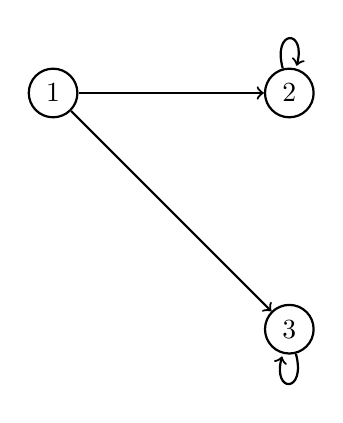
\begin{tikzpicture}[->, auto, node distance=3cm, thick]
    % Define states
    \node[circle, draw] (A) {1};
    \node[circle, draw, right of=A] (B) {2};
    \node[circle, draw, below of=B] (C) {3};

    % Transitions between states
    \draw (A) edge (B);
    \draw (A) edge (C);
    % \draw (C) edge (A);

    % Self-loops
    % \draw (A) edge[loop above] (A);
    \draw (B) edge[loop above] (B);
    \draw (C) edge[loop below] (C);

    \end{tikzpicture}
    \caption{Graph of a reducible Markov chain with two closed communication classes. Note that we might end up stuck at either state $2$ or state $3$.}
    \label{fig:markov_chain_two_closed_classes}
\end{figure}

Clearly, we have two stationary probability distributions with all their weight in either state $2$ or state $3$. Once again, our intuition tells us we might require an irreducible Markov chain.

Now it's time to specify our intuitions precisely. The following result regarding irreducible aperiodic Markov chains is very significant.

\begin{theorem}[Positive n-Step Transition Matrix for Irreducible Aperiodic Markov Chains]
    For every irreducible aperiodic Markov chain specified by $\bm{P}$, there exists an $m \in \mathbb{N}_{>0}$ s.t. $\bm{P}^m > \bm{0}$, where the comparison is element-wise.
    \label{theorem:positive_transition_matrix}
\end{theorem}

We first prove the following auxiliary lemma:

\begin{lemma}
    Let $i \in S$ be an aperiodic state. Then there exists an $L \in \mathbb{N}$ s.t. for all $n > L: (\bm{P}^n)_{ii} > 0$.
    \label{lemma:aux}
\end{lemma}
\vspace{-2.5em}
\begin{proof}
    Since state $i$ is aperiodic, we can find $n_1, \dots, n_r \in \mathbb{N}$ s.t. $(\bm{P}^{n_1})_{ii} > 0, \dots, (\bm{P}^{n_r})_{ii} > 0$ and $\gcd \{ n_1, \dots , n_r \} = 1$. From number theory, we know that for $L \coloneqq \prod_{k=1}^{r} n_k$ we can write every natural number $n > L$ in the form $n = l_1 n_1 + \dots + l_r n_r$ for suitable $l_1, \dots, l_r \in \mathbb{N}$. Hence:
    \[
        (\bm{P}^{l_1 n_1 + \dots + l_r n_r})_{ii} \geq ((\bm{P}^{n_1})^{l_1})_{ii} \cdot \dots \cdot ((\bm{P}^{n_r})^{l_r})_{ii} > 0 \quad .
    \]
\end{proof}

\begin{remark}
    \label{remark:converse_lemma_aux}
    The converse of lemma~\ref{lemma:aux} is also true for obvious reasons.
\end{remark}

\begin{proof}[Proof of Theorem~\ref{theorem:positive_transition_matrix}]
    Let $L'$ be defined as the maximum of all $L$ defined like in Lemma~\ref{lemma:aux} when looping over all $i \in S$. Then for every $n > L'$, we have that $\bm{P}^n$ has positive entries along its diagonal. It follows that if $(\bm{P}^{t_{ji}})_{ij} > 0$ for some $t_{ji} \in \mathbb{N}_{>0}$, then we have $(\bm{P}^{n + t_{ji} + \tau})_{ij} > 0$ as well for every $\tau \in \mathbb{N}$. Furthermore, for every $i,j \in S$ we have $(\bm{P}^{t_{ji}})_{ij} > 0$ at some point $t_{ji} \in \mathbb{N}_{>0}$ since $\bm{P}$ is irreducible. Hence, at some point all the zeros must have vanished.
\end{proof}

\begin{corollary}
    Once $\bm{P}^m > \bm{0}$, then for all $\tau \in \mathbb{N}: \bm{P}^{m + \tau} > \bm{0}$. 
\end{corollary}

The reader might question the importance of Theorem~\ref{theorem:positive_transition_matrix}. Clearly, we can see the interplay of the two properties of the Markov chain being irreducible and aperiodic in the proofs. But how does it help us finding a stationary probability distribution? Well, to answer this, we need another fundamental result, which we will cover next.


\subsection{Perron-Frobenius Theorem}
To come straight to the point, the Perron-Frobenius Theorem reads as follows:

\begin{theorem}[Perron-Frobenius]
    \label{theorem:perron_frobenius}
    Let \( \bm{A} \) be a non-negative matrix (i.e., all entries of \( \bm{A} \) are non-negative) with the propetry that there exists some \( m \in \mathbb{N} \) such that all entries of \( \bm{A}^m \) are strictly positive. Then the following hold:

    \begin{enumerate}
        \item The matrix \( \bm{A} \) has a unique largest non-negative eigenvalue \( \lambda_{\max} \), and this eigenvalue is simple (it has algebraic multiplicity 1).
        \item The eigenvalue \( \lambda_{\max} \) is real and positive.
        \item There is a corresponding positive eigenvector \( \bm{v}^* \) (i.e., all entries of \( \bm{v}^* \) are positive) associated with \( \lambda_{\max} \).
        \item Any other eigenvalue \( \lambda \) of \( \bm{A} \) satisfies \( |\lambda| < \lambda_{\max} \).
    \end{enumerate}
\end{theorem}

This is a mouthful, and we will not prove this theorem in this general form, as it is not trivial to do so. Instead, we focus on the case of $\bm{A}$ being a Markov chain transition matrix, meaning all columns sum to $1$. To this end, we will write $\bm{P}$ again instead of $\bm{A}$. Additionally, we assume $\bm{P}$ to be strictly positive. Furthermore, we will not provide a rigorous proof, but we will lay the foundation for an intuitive understanding.

\begin{proof}[Proof of Perron-Frobenius for Positive Markov Chain Transition Matrices]
    ~\\
    Consider the mapping $T: \Delta \to \Delta$ from the unit simplex $\Delta$ onto itself defined by $T(\bm{v}) \coloneqq \bm{Pv}$. We want to show that $T$ is a contraction mapping with respect to the $L_1$ norm. We do this step last in order to understand the line of argument better.
    
    Thus, assume that $T$ is a contraction mapping with respect to the $L_1$ norm. By the \textsc{Banach Fixed-Point Theorem} we know that this mapping has a \emph{unique} fixed point $\bm{v}^*$. We see that $\bm{v}^*$ is an eigenvector of $\bm{P}$ with eigenvalue $\lambda = 1$. Clearly, $\bm{v}^*$ is positive and is the only eigenvector with non-negative entries, as if there were another one say $\bm{v}'$, then $\frac{\bm{v}'}{\|\bm{v}'\|_1}$ must be one as well, but this point lies on $\Delta$, hence it must have an eigenvalue of $1$ and must be a fixed point of $T$, a contradiction to the uniqueness of $\bm{v}^*$.

    So every other eigenvector $\bm{w}$ with eigenvalue $\mu$ must have a coordinate-entry which is negative or truly complex. Write $|\bm{w}|$ for the vector with coordinates $|\bm{w}_j|$. The computation
    \[
        |\mu||\bm{w}|_i = |\mu \bm{w}_i| = |\sum_{j} \bm{P}_{ij} \bm{w}_j| \leq \sum_{j} |\bm{P}_{ij}| |\bm{w}_j| = \sum_{j} \bm{P}_{ij} |\bm{w}_j| = (\bm{P} |\bm{w}|)_i
    \]
    shows that $|\mu| \|\bm{w}\|_1 \leq \|\bm{P} |\bm{w}|\|_1 = \|\bm{w}\|_1$ and hence $|\mu| \leq 1$. Now, the final trick is that we can assume the "$\leq$" in the equation above to actually be "$<$".

    To see this, note that we only have equality iff all entries of $\bm{w}$ are on a line in the complex plane, i.e. we can write $\bm{w} = c |\bm{w}|$ for some $c \in \mathbb{C}, |c| = 1$. This would mean that $\bm{P} \bm{w} = \bm{P} c |\bm{w}| = c \bm{P} |\bm{w}| \overset{!}{=} \mu \bm{w}$. Hence, $\bm{P} |\bm{w}| = \frac{\mu}{c} \bm{w} = |\frac{\mu}{c}| |\bm{w}|$. Thus, we must have $|\bm{w}| = \bm{v}^*$ and $|\mu| = |c| = 1$ as already discussed. Hence, $\bm{w} = c \bm{v}^*$ (and $\mu = 1$), which is just a different representation of the eigenvector $\bm{v}^*$ already found. So for every eigenvector $\bm{w}$ other than $\bm{v}^*$ with eigenvalue $\mu$ we must have that $|\mu| < 1$.

    \smallskip
    Now, the only thing left to do is to show that $T$ is in fact a contraction mapping. To this end, we must find a $0 \leq k < 1$ s.t. for all $\bm{x}, \bm{y} \in \Delta$ we have
    \[
        \|T(\bm{x}) - T(\bm{y})\|_1 = \|\bm{P} (\bm{x} - \bm{y})\|_1 \leq k \|\bm{x} - \bm{y}\|_1 \quad .
    \]
    The idea is that $T$ maps from $\Delta$ into a real subspace $\Delta_{\bm{P}} \subsetneq \Delta$ defined by the simplex spanned by the columns of $\bm{P}$, which we call the vertices of the simplex $\Delta_{\bm{P}}$. $\Delta_{\bm{P}}$ does not contain any of the border points of $\Delta$. Applying $T$, we see that $T^2$ maps into an even smaller sub-simplex $\Delta_{\bm{P}^2} \subsetneq \Delta_{\bm{P}}$, and so on and so forth.

    Formally, we define $k$ as $k \coloneqq \frac{\|\Delta_{\bm{P}}\|_1}{2}$, where $\|\Delta_{\bm{P}}\|_1$ denotes the maximum $L_1$ distance between any points in $\Delta_{\bm{P}}$. We can always measure this distance at two of the vertices of the simplex, as both the $L_1$ norm and the simplex are convex, so the maximum will be reached at vertices. But since all coordinates of all vertices are strictly positive, we have $\|\Delta_{\bm{P}}\|_1 < 2$, so $k$ is in fact valid.

    Now, for the sake of contradiction, assume $\|\bm{P} (\bm{x} - \bm{y})\|_1 > k \|\bm{x} - \bm{y}\|_1$ for some $\bm{x}, \bm{y} \in \Delta$. Note that $\bm{x} - \bm{y}$ is a vector with entries which sum to $0$, which defines a direction tangent to the unit simplex $\Delta$. We can always find two points $\bm{x}', \bm{y}' \in \Delta$ with the same direction and $\|\bm{x}' - \bm{y}'\|_1 = 2$ (one point will be a vertex, the other will lay on the opposite side). Hence:
    \begin{align*}
        \|\bm{P} (\bm{x}' - \bm{y}')\|_1 &= \frac{\|(\bm{x}' - \bm{y}')\|_1}{\|(\bm{x} - \bm{y})\|_1} \|\bm{P} (\bm{x} - \bm{y})\|_1 \\
        &> k \frac{\|(\bm{x}' - \bm{y}')\|_1}{\|(\bm{x} - \bm{y})\|_1} \|\bm{x} - \bm{y}\|_1 \\
        &= k \|(\bm{x}' - \bm{y}')\|_1 = 2k = \|\Delta_{\bm{P}}\|_1 \quad , \\
    \end{align*}
    a contradiction.
\end{proof}

\begin{corollary}
    Based on the proof, we see that for every $\bm{v} \in \Delta: \lim_{n \to \infty} \bm{P}^n \bm{v} = \bm{v}^*$. Now, set $\bm{v} \coloneqq \bm{e_i}$. It follows that $\lim_{n \to \infty} \bm{P}^n = \bm{P}_{\bm{v}^*}$, where $\bm{P}_{\bm{v}^*}$ is the matrix whose columns all consist of the unique fixed point $\bm{v}^*$. This convergence is independent of the norm.
\end{corollary}

\begin{lemma}[Assuming a Positive Matrix is not a Restriction]
    If the Perron-Frobenius Theorem holds for positive matrices, then it also holds for non-negative matrices $\bm{A}$ with the property that there exists an $m \in \mathbb{N}$ s.t. $\bm{A}^m > \bm{0}$.
\end{lemma}
\vspace{-2.5em}
\begin{proof}
    Let $\lambda_1, \dots, \lambda_n$ by the eigenvalues of $\bm{A}$ allowing for multiplicity and ordering them s.t. $|\lambda_1| \geq \dots \geq |\lambda_n|$. Per definition, we know there exists an $m \in \mathbb{N}$ s.t. $\bm{A}^m > \bm{0}$. Also, for every $\tau \in \mathbb{N}$ we have $\bm{A}^{m + \tau} > \bm{0}$. We apply the Perron-Frobenius Theorem on $\bm{A}^{m + \tau}$ to get the eigenvalues $\lambda_1^{(\tau)}, \dots, \lambda_n^{(\tau)}$ s.t. $\lambda_1^{(\tau)} > |\lambda_2^{(\tau)}| \geq \dots \geq |\lambda_n^{(\tau)}|$. Now, assume that we have ordered $\lambda_1, \dots, \lambda_n$ perefectly s.t. $\lambda_i^{m + \tau} = \lambda_i^{(\tau)}$, as such an order always exists. From this, we immediately see that $|\lambda_1|$ is strictly bigger than all other eigenvalues of $\bm{A}$. It also must be real and positive, as both $\lambda_1^{(0)}$ and $\lambda_1^{(1)}$ are real and positive, and thus $\lambda_1 = \frac{\lambda_1^{(1)}}{\lambda_1^{(0)}}$ is real and positive. So statements (1), (2), and (4) of theorem~\ref{theorem:perron_frobenius} follow.

    Let $\bm{v}^{\tau}$ be the eigenvector of $\bm{A}^{m + \tau}$ with eigenvalue $\lambda_1^{(\tau)}$. By the Perron-Frobenius theorem we know that $\bm{v}^{\tau}$ is positive. Also, we know that $\bm{A}$ has an eigenvector $\bm{v}^*$ with eigenvalue $\lambda_1$, since $\lambda_1$ is unique. This eigenvector will not change for $\bm{A}^r$ for every $r \in \mathbb{N}$, and the only matching eigenvector for $\bm{v}^*$ when $r = m + \tau$ is $\bm{v}^{\tau}$ based on the eigenvalues. And hence $\bm{v}^* \coloneqq \bm{v}^{\tau}$ itself is positive, which was the last claim (3).
\end{proof}

\begin{corollary}
    The Perron-Frobenius Theorem holds for irreducible aperiodic Markov chain transition matrices $\bm{P}$, and $\lambda_{max} = 1$. The associated eigenvector is the stationary probability distribution $\bm{\mu}$.
\end{corollary}

\begin{remark}
    $T: \Delta \to \Delta, T(\bm{v}) \coloneqq \bm{Pv}$ is not a contraction mapping in general for irreducible aperiodic Markov chain tranisition matrices $\bm{P}$. But we still have $\Delta_{\bm{P}^{r+1}} \subsetneq \Delta_{\bm{P}^{r}}$, so intuitively $T^{r}(\bm{v}) = \bm{P}^r\bm{v}$ itself will converge to $\bm{\mu}$. To formally prove this, let $m \in \mathbb{N}$ be s.t. $\bm{P}^m > \bm{0}$. Then also $\bm{P}^{m + 1} > \bm{0}$. $((\bm{P}^m)^r)_{r \in \mathbb{N}}$ and $((\bm{P}^{m + 1})^r)_{r \in \mathbb{N}}$ have the common subsequence $((\bm{P}^{m^2 + m})^r)_{r \in \mathbb{N}}$ and hence must converge to the same $\bm{P_\mu}$. From this, it follows that $(\bm{P}^r)_{r \in \mathbb{N}}$ itself converges to $\bm{P_\mu}$.
\end{remark}

\begin{remark}
    \label{remark:exponential_decay}
    Again, let $m \in \mathbb{N}$ be s.t. $\bm{P}^m > \bm{0}$. Based on the proof, we see that
    \[
        \| \bm{P}^{mr} \bm{v} - \bm{\mu} \|_1 \leq \dfrac{\|\Delta_{\bm{P^m}}\|_1^r}{2^r} \| (\bm{v} - \bm{\mu}) \|_1 \in \mathcal{O} \left( \left[ \frac{\|\Delta_{\bm{P^m}}\|_1}{2} \right] ^r \right) \quad .
    \]
    In other words, we have \emph{exponential decay} in the distance between $\bm{P}^{mr} \bm{v}$ and $\bm{\mu}$ with respect to $r$. Hence, we also have
    \[
        \| \bm{P}^{r} \bm{v} - \bm{\mu} \|_1 \in \mathcal{O} \left( \left[ \frac{\|\Delta_{\bm{P^m}}\|_1}{2} \right] ^{\dfrac{r}{m}} \right) = 
        \mathcal{O} \left( \left[ \left( \frac{\|\Delta_{\bm{P^m}}\|_1}{2} \right) ^{\dfrac{1}{m}} \right] ^r \right) \quad .
    \]
\end{remark}

\begin{hypothesis}
    Maybe
    \[
        \lim_{m \to \infty} \left[ \|\Delta_{\bm{P^m}}\|_1 \right] ^{\frac{1}{m}}
    \]
    evaluates to something interesting like $|\lambda_2|$ of $\bm{P}$, or equivalently $\lim_{m \to \infty}: |\lambda_2^{(m)}|^{\frac{1}{m}} = \|\Delta_{\bm{P^m}}\|_1^\frac{1}{m}$ where $\lambda_2^{(m)}$ is the second largest eigenvalue of $\bm{P}^m$. Maybe in the proof there is another (complex) eigenvector hidden. Maybe we also use another norm, as we have convergence independent of the norm, but the contraction mapping is not as trivial.
\end{hypothesis}

\end{document}